\documentclass[12pt]{article}

% Packages 
\usepackage{amsmath}
\usepackage{datetime}
\usepackage{graphicx}
\usepackage{listings}
\usepackage{gensymb}

\graphicspath{{./images/}}

\newdate{date}{03}{05}{2022}
\title{
    Final Project

    \large{
        ME EN 6240 Advanced Mechatronics
    }  
}
    
\author{
        Ryan Dalby
}
\date{\displaydate{date}}

\setlength\parindent{0pt}

\begin{document}
\maketitle

\section*{1.}
\textit{The NU32 communicates with the encoder counter by an SPI channel. Which SPI channel will you use? Which NU32 pins does it use?}

\begin{center}
\begin{tabular}{|c|c|c|}
    \hline
    Pin Name & NU32 Pin & PIC32 Pin \\
    \hline
    SCK2 & G6 & 4\\
    SDI2 & G7 & 5\\
    SDO2 & G8 & 6\\
    \hline
    SCK3 & D1 & 49\\
    SDI3 & D2 & 50\\
    SDO3 & D3 & 51\\
    \hline
    SCK4 & B14 & 29\\
    SDI4 & F4 & 31\\
    SDO4 & F5 & 32\\
    \hline
\end{tabular}
\end{center}

On the NU32 SPI2 is unavailable because RG6 and RG7 are used for UART communication with with host computer.
Thus SPI3 and SPI4 can be used on the NU32 but I will choose SPI4 as it seems to overlap with less lower number digital IO pins than SPI3 which would generally be the first used for other things.

This means I will use NU32 pins (PIC32 in parenthesis) B14(29) for SCK4, F4(31) for SDI4, and F5(32) for SDO4.

% Note in examples B8 (21) is often used for SS4


\section*{2.}
\textit{The NU32 reads the MAX9918 current sensor using an ADC input. Which ADC input will you use? Which NU32 pin is it?}

I will choose to use AN5 which corresponds to B5 on the NU32 (pin 11 on the PIC32) as an analog input to the PIC32 for the MAX9918 current sensor.

% AN5 was often used for ADC examples and problems during this class.

\section*{3.}
\textit{The NU32 controls the DRV8835 H-bridge using a direction bit (a digital output) and PWM (an output compare and a timer). Which peripherals will you use, and which NU32 pins?}

% For the direction bit I will use digital output configured RB7 which corresponds to B7 on the NU32 (pin 18 on the PIC32). 
% This can be changed if there are conflicts or another unused digital pin makes wiring easier, but this one was chosen since it has limited possible conflicts.
For the direction bit I will use digital output configured RD1 which corresponds to D1 on the NU32 (pin 49 on the PIC32). 
This was chosen because of its close physical proximity on the NU32 to the chosen output compare.

For PWM I will plan on using output compare 1 (OC1) which corresponds to D0 on the NU32 (pin 46 on the PIC32).
For the output compare modules I will use timer2 as only timer2 and timer3 are options.
If a higher range of values are needed then timer23 will be used.

\section*{4.}
\textit{Which timers will you use to implement the 200 Hz position control ISR and the 5 kHz current control ISR? What priorities will you use?}

Since the period of the control loops are faster than the maximum countable time before 16-bit timer rollover it should be okay to use sing 16-bit timers for both control loops.
I will use timer4 for the 200 Hz position control ISR and timer5 for the 5 kHz current control ISR. 
If a 32-bit timer for a loop is needed I can use timer45 and then use timer1 for the other loop.
If two 32-bit timers are needed this won't really be possible because timer23 will be being used for PWM.

I will give both ISRs for position and current control the same priority so neither will interrupt each other once one begins and give a higher subpriority to the position control ISR since it occurs less often and I would like to make sure when it needs to execute it will be ahead of the current control ISR which occurs much more frequently.
% Prof suggests current control priority above position...

\section*{5.}
\textit{Based on your answers to these questions, and your understanding of the project, annotate the block diagram of Figure 27.7. Each block should clearly indicate which devices or peripherals perform the operation in the block, and each signal line should clearly indicate how the signal is carried from one block to the other. (After this step, there should be no question about the hardware involved in the project. The details of wiring the H-bridge, current sensor, and encoder are left to later.)}

\begin{center}
    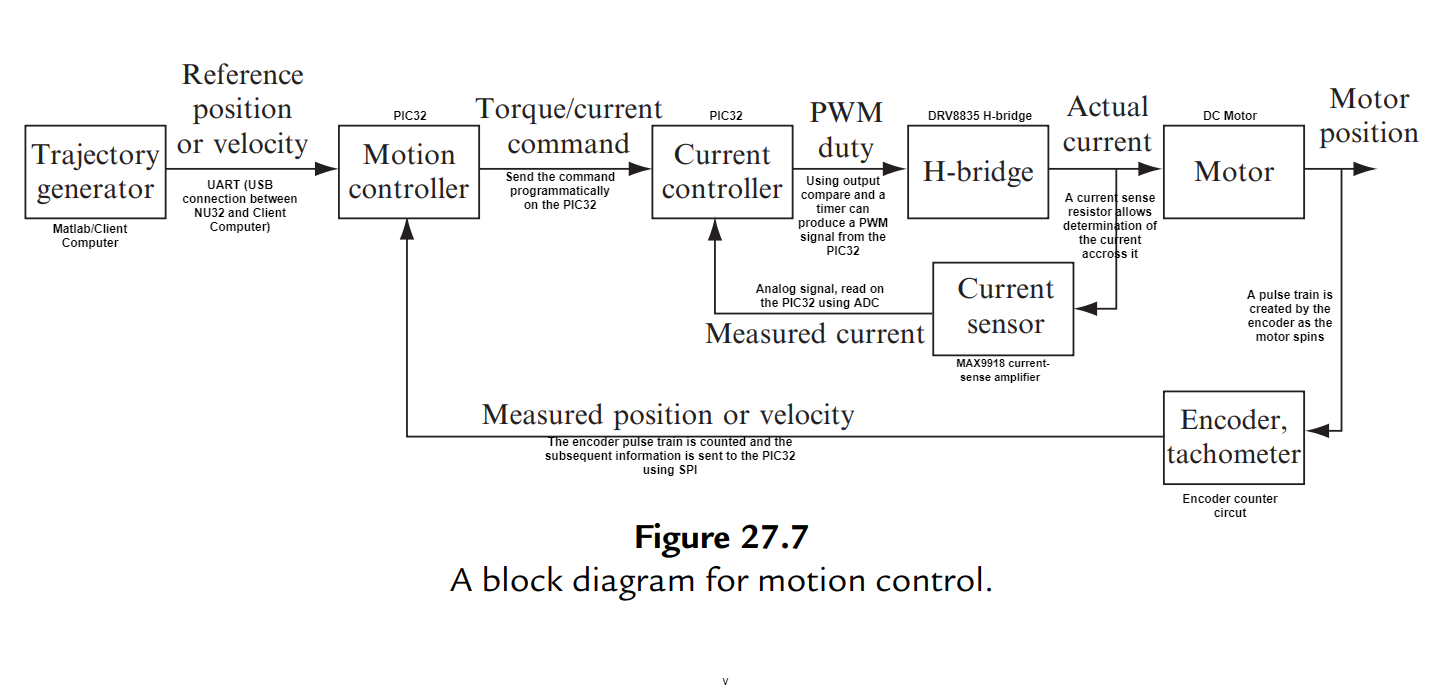
\includegraphics[width=5.2in]{fig27_7_labelled.png}
\end{center}

\section*{6.}
\textit{Based on which circuit boards need to be connected to which pins of the NU32, and the connections of the circuit boards to the motor and encoder, sketch a proposed layout of the circuit boards relative to the NU32 so that wire crossing is approximately minimized. (Do not make a full circuit diagram at this time.)}

Note the circuit diagram for the NU32 shown below does not exactly match the physical NU32, likely it is a slightly different iteration of the NU32. 
Still it allows the sketch to get the idea of what connections are needed across.

\begin{center}
    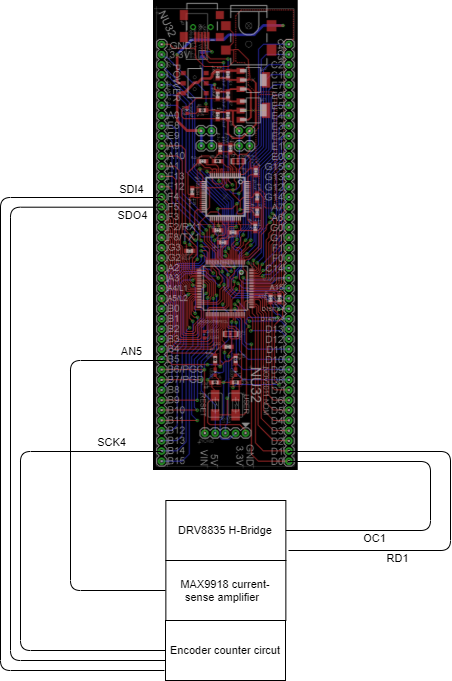
\includegraphics[width=4in]{circuit_sketch.png}
\end{center}

\section*{7.}
\textit{Turn in a circuit diagram showing all connections of the H-bridge to the NU32, motor, and current sensor PCB.}

\section*{8.}
\textit{Turn in your best ITEST plot, and indicate the control gains you used, as well as their units.}

\section*{9.}
\textit{Turn in your best plots of following the step and cubic trajectories in Figure 28.5 with the load attached. Indicate the control gains you used, as well as their units.}

\section*{10.}
\textit{Turn in all your code for the motor control project.}

\section*{11.}
\textit{Turn in a video demonstration of the motor control project.  The demonstration should include the following:}
\begin{enumerate}
    \item[1.]
    \textit{Startup the system (initialization etc.)}

    \item[2.]
    \textit{Show the position step response using “good” gains of the controller}

    \item[3.]
    \textit{Change the PID gains to show a “bad” position step response}

    \item[4.]
    \textit{Change back to good gains and cubic trajectory tracking}
\end{enumerate}


\section*{Miscellaneous Notes}
Step 5:

Choose $R_3 = 220 \Omega$

$V = 6V$ % Four 1.5v batteries in series
$R_{motor} = 4.6 \Omega$
$I_{max} = 2V/R_{motor} = 2(6)/(4.6) = 2.61A$ % Worst case change from -V to +V
$V_{max} = I_{max} (15 m\Omega) = (2.61) (15 \times 10^{-3}) = 0.04 V$

$1.65 = G \times V_{max} = (1+\frac{R_1}{R_2}) (0.04)$

$G = 41.25$

$\frac{R_2}{R_1} = 40.25$

Choose $R_2 = 330 k\Omega$ and $R_1 = 10 k\Omega$.
Thus $G = 33$

$f_c = \frac{1}{2 \pi RC} \approx 200 Hz$

% Choose $R = 1 M\Omega$ and $C = 1000 pF$.
% Thus $f_c = 159 Hz$
Choose $R = 680 \Omega$ and $C = 1 \mu F$.
Thus $f_c = 234 Hz$


Calibration (input voltage )
% \begin{center}
% \begin{tabular}{|c|c|c|c|}
%     \hline
%     Input Voltage & R0 & Expected Current & Measured Current\\
%     \hline
%     5V & 10 & 0.5 A & 0.390 A\\
%     \hline
%     -5V & 10 & 0.5 A &  -0.370 A\\
%     \hline
%     5V & 20 & 0.25 A & 0.205 A \\
%     \hline
%     -5V & 20 & -0.25 A & -0.200 A \\
%     \hline
%     5V & 40 & 0.125 A & 0.106 A \\
%     \hline
%     -5V & 40 & -0.125 A & -0.109 A \\
%     \hline
% \end{tabular}
% \end{center}

\begin{center}
\begin{tabular}{|c|c|c|c|c|}
    \hline
    Input Voltage & R0 & Expected Current & Measured Current & ADC Counts \\
    \hline
    6V & 40 & 150 mA & 130 mA & 568 574 528 \\
    \hline
    -6V & 40 & -150 mA & -120 mA & 448 512 528\\
    \hline
    6V & 30 & 200 mA & 160 mA & 575 560 512 \\
    \hline
    -6V & 30 & -200 mA & -160 mA & 495 415 447 \\
    \hline
    6V & 20 & 300 mA & 220 mA & 591 471 576 \\
    \hline
    -6V & 20 & -300 mA & -230 mA & 391 464 448 \\
    \hline
    6V & 10 & 600 mA & 430 mA & 608 607 623 \\
    \hline
    -6V & 10 & -600 mA & -440 mA & 439 415 464 \\
    \hline
    0 V & 0 & 0 mA & 0 mA & 503 512 511 \\
    \hline
\end{tabular}
\end{center}

\begin{center}
    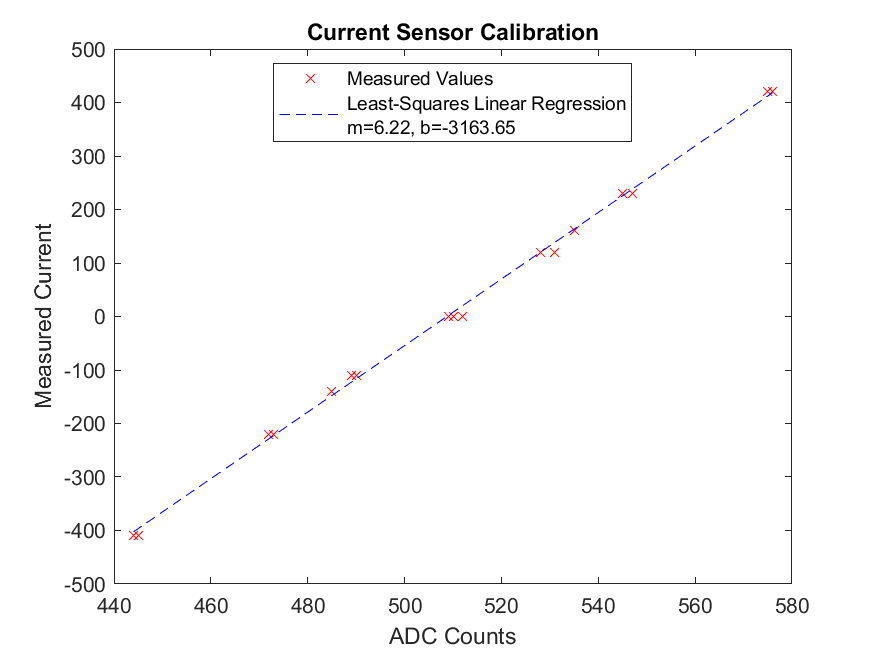
\includegraphics[width=5in]{current_sensor_calibration_curve.png}
\end{center}

\end{document}